\documentclass[a4paper,12pt]{report}

%--------------------------------------
% The cmap package creates a ToUnicode mapping in the PDF, which
% ensures that internal character codes (e.g., for Cyrillic text)
% are correctly translated to Unicode when copying from the PDF.
% Without it, copy-paste operations may yield garbled text.
\usepackage{cmap}
\usepackage[T2A]{fontenc}
\usepackage[utf8]{inputenc}
\usepackage[english, russian]{babel}
%--------------------------------------

% размеры полей из ГОСТ 7.32-2017.pdf п.6.1.1
\usepackage[
	left=30mm,
	right=15mm,
	top=20mm,
	bottom=20mm,
	headsep=0pt,
	includefoot
]{geometry}

% абзацный отступ из ГОСТ 7.32-2017.pdf п.6.1.1
\setlength{\parindent}{1.25cm}

% fix overfull hboxes
\emergencystretch=1cm

% for \texttt and other math
\usepackage{amsmath}

\usepackage{graphicx}
\graphicspath{ {./assets/} }

\usepackage{subcaption}

\usepackage{biblatex}
\addbibresource{references.bib}

\begin{document}

\begin{titlepage}
  \begin{center}
    ФЕДЕРАЛЬНОЕ ГОСУДАРСТВЕННОЕ БЮДЖЕТНОЕ ОБРАЗОВАТЕЛЬНОЕ УЧРЕЖДЕНИЕ ВЫСШЕГО ОБРАЗОВАНИЯ

    <<МОСКОВСКИЙ ГОСУДАРСТВЕННЫЙ УНИВЕРСИТЕТ

    имени М.В.ЛОМОНОСОВА>>

    \vspace{0.7cm}

    МЕХАНИКО-МАТЕМАТИЧЕСКИЙ ФАКУЛЬТЕТ

    \vspace{0.7cm}

    КАФЕДРА ВЫЧИСЛИТЕЛЬНОЙ МАТЕМАТИКИ

    \vspace{3cm}

    ВЫПУСКНАЯ КВАЛИФИКАЦИОННАЯ

		РАБОТА СПЕЦИАЛИСТА

    \vspace{0.7cm}

    \textbf{Геометрические построения с использованием}

		\textbf{нейросетевых технологий}

  \end{center}

  \vspace{2cm}

  \hfill
  \begin{minipage}{0.5\textwidth}
    Выполнил студент

    631 академической группы 

    Шерстобитов Андрей Сергеевич

    \vspace{1cm}

    \underline{\hspace{4cm}}

    подпись студента

    \vspace{0.5cm}

    Научный руководитель:

    к.ф.-м.н, доцент 

    Валединский Владимир Дмитриевич

    \vspace{1cm}

    \underline{\hspace{4cm}}

    подпись научного руководителя
 \end{minipage}

  \vfill

  \begin{center}
    \large Москва

    \the\year
  \end{center}

\end{titlepage}


\tableofcontents

\chapter{Введение}

Восстановление трехмерных моделей (далее — 3D-моделей) — одна из наиболее
популярных задач компьютерного зрения и графики. Цифровое представление и
воссоздание трехмерных сцен на компьютере лежит в основе множества важных
приложений, а в последние годы 3D-реконструкция стала особенно актуальной
благодаря увеличению вычислительных мощностей графических ускорителей и
последующему ускоренному развитию машинного обучения и нейронных сетей.
Современные методы способны получать объемные модели высокой точности из
ограниченного набора изображений (далее — датасетов), что открывает пути к
упрощенному созданию фотореалистичных виртуальных миров и цифровых копий
реальных объектов.

Задача автоматического построения 3D-модели по ограниченному количеству снимков
крайне востребована: она позволяет отказаться от ручного моделирования и
непосредственного физического копирования объектов. Технологии 3D-реконструкции
находят применение в самых разных сферах: от развлечений (игры, кино,
виртуальная реальность), медицины (моделирование органов по снимкам для
подготовки операций), робототехники (построение карты окружения для навигации)
до промышленного дизайна и инженерии (создание точных цифровых моделей изделий
для проектирования). Таким образом, тема реконструкции 3D-моделей с помощью
нейросетей является актуальной благодаря как научному интересу, так и огромному
практическому потенциалу во множестве отраслей.

В настоящее время существуют различные подходы к 3D-реконструкции: традиционные
методы (стереозрение, многовидовая реконструкция, фотометрические и активные
методы сканирования) и современные нейросетевые методы (генеративные модели,
обучаемые многовидовые методы, нейронные радиационные поля — NeRF и их
модификации). Каждый из этих подходов обладает своими преимуществами и
ограничениями, которые важно учитывать при выборе оптимального решения.

Целью данной работы является исследование современных нейросетевых методов
3D-реконструкции и разработка эффективного подхода для решения задач
с различными требованиями к точности и доступности вспомогательного
оборудования. Достижение поставленной цели предусматривает решение ряда
взаимосвязанных задач:

\begin{enumerate}
	\item Проанализировать текущее состояние области 3D-восстановления, описать
	традиционные методы и методы, использующие нейронные сетей.  Рассмотреть
	обзорные источники, так и конкретные передовые разработки. Систематизировать
	подходы, их преимущества и недостатки.
	\item Выбрать два нейросетевых метода 3D-реконструкции для двух
	контрастирующих задач. Обосновать выбор каждого из методов.
	\item Подготовиться к использованию выбранных методов. Если потребуется,
	сгенерировать соответствующие данных для обучения и подобрать гиперпараметры
	нейронной сети.
	\item Провести эксперимент, оценить качество восстановленной геометрии и
	фотореалистичность визуализации, требования к объему исходных данных, время
	обучения модели и генерации результатов.
	\item Проанализировать полученные
	результаты, определить сильные и слабые стороны каждого из методов. Сделать
	выводы о том, какой подход в наибольшей степени отвечает поставленной цели и
	как их можно комбинировать или улучшить.
\end{enumerate}

Таким образом, исследование позволит получить представление о
возможностях современных нейросетевых подходов к 3D-реконструкции, определить
оптимальные алгоритмы для решения практических задач, а также выявить
направления для дальнейших улучшений и развития методов автоматического
восстановления трехмерных сцен.

\chapter{Теоретический обзор методов восстановления 3D-моделей}

\section{Постановка задачи 3D-восстановления}

Качественно выполненная огранка драгоценного камня существенно повышает
стоимость ювелирного изделия, в то же время неправильная огранка негативно
влияет на эстетическое восприятие. Для минимизации человеческого
фактора и для ускорения процесса желателен нейросетевой метод реконструкции,
который мог бы использовать серию снимков для автоматического получения
высокоточной трехмерной модели камня. Это позволяет мастеру мгновенно сравнивать
получаемый результат с исходной моделью и оперативно корректировать действия для
достижения идеальной формы.

В то же время, в археологии имеются принципиально иные предпосылки для задачи
восстановления трехмерных моделей. Здесь трехмерная реконструкция нужна не
столько для достижения точности соответствия эталонной геометрии, сколько для
идентификации личности по черепу, изучения анатомических особенностей,
проведения антропологических исследований и судебно-медицинских экспертиз. Целью
является реконструкция полной и детализированной модели объекта, даже если
исходные данные неполны или повреждены. Метод должен быть устойчив к шумам и
потерям информации, и при этом позволять визуализировать максимально
информативную трехмерную модель.

Противопоставляя две эти задачи, следует отметить, что восстановление геометрии
драгоценного камня требует высокой точности и низкой погрешности реконструкции. В то же
время, реконструкция археологического объекта, такого как череп, направлена
прежде всего на целостность и реалистичность итоговой модели, которая будет
использоваться в дальнейших экспертных исследованиях и идентификации, где точное
соответствие исходной форме не всегда возможно и не является основной целью.

Таким образом, для эффективного решения обеих задач необходимы различные подходы
к трехмерному моделированию: для огранки камней приоритетом является
высокоточная геометрическая реконструкция, в то время как в археологической
задаче реконструкции черепов важна полная, визуально реалистичная модель,
способная корректно отразить исходную структуру и особенности, даже в условиях
частичной потери исходных данных.

\section{Традиционные и современные подходы}

\subsection{Стереоскопическое изображение (стереопара)}

Стереоскопическая съемка (\cite{ussr1981phototech}) основана на использовании
двух съёмочных систем (или двух изображений), фиксирующих сцену с разных точек.
Такая система позволяет определить относительное положение предметов по признаку
параллакса — смещению изображения объектов ближнего плана относительно фона при
изменении точки наблюдения.  Основная задача — определить пары соответствующих
точек на левом и правом изображениях и вычислить так называемое смещение (англ.
disparity), т. е.  разность координат этих точек вдоль горизонтальной оси.
Расстояние до объекта (глубина сцены) $Z$ обратно пропорционально смещению: $Z =
\frac{f \cdot B}{d}$, где $f$ — фокусное расстояние объектива, $B$ — база
(расстояние между оптическими осями камер), $d$ — смещение.

Также стереометрические методы опираются на законы эпиполярной геометрии,
согласно которым соответствующие точки лежат на эпиполярных линиях, взаимное
расположение которых описывается фундаментальной матрицей (\cite{Hartley:2003:MVG:861369}).

В простейших реализациях применяются методы блочного сравнения (например, по
критерию суммы квадратов отклонений, коэффициенту взаимной корреляции и др.).
Более совершенные методы используют глобальную оптимизацию (например, на основе
динамического программирования, графовых моделей и пр.). Каждый из предложенных
развитий метода несет свои достоинства и недостатки
(\cite{kok2019reviewonsterevision}). Рассмотрим достоинства и ограничения
для алгоритма в общем случае.

\textbf{Достоинства:} стереофотограмметрия сравнительно легко реализуема и
хорошо изучена. Такие методы широко применяются, в том числе в навигации и
системах помощи водителю, а также в киноиндустрии. Современные алгоритмы
достигают высокой точности (точность сопоставления превышает 95\%,
\cite{fsian2022comparisonstereomatchingalgorithms}).

\textbf{Недостатки:} метод требует наличия перекрывающихся изображений и
наличия текстуры. В однородных или повторяющихся участках возникают ошибки
сопоставления. Также проблемы возникают на границах объектов (из-за взаимных
затенений, англ. occlusions), а также при съёмке прозрачных или зеркальных
объектов, где нарушается фотометрическое соответствие. Методы
стереофотограмметрии, как правило, предполагают ламбертов характер отражения,
что делает их неприменимыми для оптически сложных поверхностей.

\subsection{Многовидовая реконструкция (Multi-View Stereo, MVS)}

Методы многовидового восстановления пространственной формы сцены (англ.
Multi-View Stereo, сокращённо MVS) представляют собой обобщение
стереоскопических методов на случай более чем двух изображений ($>2$). Целью
является построение плотной трёхмерной модели сцены на основе серии снимков,
полученных с различных точек обзора.

Среди направлений многовидовой реконструкции есть несколько популярных:

\begin{enumerate}
	\item Методы, основанные на построении визуальной оболочки (\cite{10.1109/34.273735})
	и дискретизации объёма объекта на элементы регулярной пространственной сетки —
	воксели. Типичные примеры: методы окрашивания вокселей (\cite{10.5555/794189.794361}),
	отсечения несогласованных частей (\cite{10.5555/898435}). Эти подходы последовательно
	исключают из объёма те области, проекции которых на снимки противоречат
	наблюдаемому изображению.

	\item Многослойные или гибридные подходы, в которых модель сцены
	представляется совокупностью параллельных пластов (\cite{10.1109/CVPR.1998.698642}).

	\item Поверхностные методы, использующие локальные участки изображения
	(`патчи') для восстановления точек /
	сеток в пространстве (\cite{10.1109/CVPR.2007.383246}).

\end{enumerate}

\textbf{Преимущества:} многовидовая реконструкция позволяет восстанавливать
детализированные трёхмерные модели сложных объектов, особенно при наличии
большого количества снимков с различными ракурсами. При благоприятных условиях
(матовые объекты, выраженная текстура, высокая точность съёмки) точность может
соперничать с результатами лазерного сканирования.

\textbf{Недостатки:} по сравнению с классическим стерео, многовидовая
реконструкция требует значительно больших вычислительных ресурсов. Поиск
соответствий выполняется сразу между несколькими изображениями, а сама задача
восстановления поверхности — в общем случае нелинейна и решается приближённо.
Также, как и в случае двухкамерной стереосъёмки, фотометрическое согласие
нарушается при съёмке прозрачных или зеркальных поверхностей, что делает такие
объекты трудновосстановимыми без специальных ухищрений.

Алгоритмы многовидовой реконструкции, как правило, предполагают, что параметры
камер (их расположение и внутренние параметры) известны заранее. Часто для их
оценки используется предварительный этап восстановления структуры сцены из
движения (см. ниже SfM).

К современным решениям, реализующим многовидовую реконструкцию,
относится, например, система COLMAP (\cite{schoenberger2016mvs}), объединяющая этапы определения параметров
камер и построения трёхмерной модели по множеству изображений в едином
автоматизированном процессе.

На испытаниях — бенчмарках — (например, \cite{Knapitsch2017}) классические методы многовидовой
реконструкции демонстрируют высокую точность для непрозрачных объектов. Однако
для восстановления геометрии прозрачных тел, таких как драгоценные камни,
традиционные подходы оказываются малоэффективными без дополнительной информации
или специальных методов.

\subsection{Томографическая реконструкция}

Томографические методы направлены на восстановление структуры объекта
по множеству его проекций. Математически задача сводится к
обращению интегральных преобразований (в частности, преобразования
Радона\footnote{ Иоганн Карл Август Радон (нем. Johann Karl August Radon; 16
декабря 1887, Дечин — 25 мая 1956, Вена) — австрийский математик.  }), решение
которых позволяет приближенно восстановить распределение функции плотности $f(x,y,z)$ объекта
по интегральным прямым вдоль пропущенных через объект лучей (\cite{book:869357}).

Томографические методы избегают проблемы окклюзии. Они реконструируют трехмерную
геометрию полупрозрачных объектов из ряда теневых изображений, соответствующих
различным положениям источника электромагнитного излучения. Томографию можно
использовать, если среда полупрозрачна относительно длины волны электромагнитного
излучения, используемого для получения данных.  Последнее требование обычно
требует использования рентгеновского излучения, как в медицинской или инженерной
компьютерной томографии (КТ). К сожалению, рентгеновская томография основана на
дорогостоящем и громоздком оборудовании и не может использоваться во многих
средах из-за соображений безопасности. Тем не менее, успешные применения
в задаче восстановления прозрачных сплошных объектов (\cite{10.1145/1179849.1179918}) и
газов (\cite{IHRKE2006484}).

\textbf{Преимущества:} такие методы позволяют восстановить не только внешнюю
поверхность, но и внутренние оптические свойства объекта — в частности,
показатель преломления в разных частях. Это делает возможным получение
высокоточной информации даже для оптически сложных объектов, где классические методы
неэффективны.

\textbf{Недостатки:} требуются специальные условия и оборудование,
известный фон или шаблон позади объекта. Классические алгоритмы томографии
предполагают большое число проекций (десятки и сотни) и чувствительны
к шуму в измерениях.

\subsection{Structure from Motion (SfM)}
\subsection{Визуальная одометрия (Visual Odometry)}
\subsection{Восстановление по силуэтам (Shape from Silhouette)}
\subsection{Фотометрические методы (Photometric Stereo)}
\subsection{Активные методы реконструкции}

\section{Нейросетевые методы 3D-реконструкции}


\chapter{Генерация данных в Blender для обучения моделей}

\section{Создание 3D-сцены и моделей в Blender}
\section{Настройка рендеринга и сбор данных}
\section{Подготовка датасета для обучения}


\chapter{Методы восстановления трехмерных моделей}

В данной главе рассматриваются различные подходы к восстановлению трехмерных
моделей по двумерным изображениям. Исследование начинается с анализа
классического подхода, основанного на методах структуры из движения (Structure
from Motion) и многовидовой стереоскопии (Multi-View Stereo), не использующего
нейросетевые технологии. Затем рассматриваются два современных нейросетевых
метода: первый основан на архитектуре \textit{TensoRF}, а второй использует
\textit{<BLANK>}. Сравнение этих подходов позволяет выявить преимущества и
ограничения применения нейросетевых технологий в задачах трехмерной
реконструкции.

Все эксперименты выполнялось на облачном экземпляре OpenStack Nova (Selectel) с
ОС Ubuntu 22.04 LTS: 2 x Intel Xeon Silver 4214R @ 2,4 ГГц (8 физических ядер),
16 ГиБ ОЗУ, GPU NVIDIA Tesla T4 с 16 ГиБ памяти и SSD-томом 100 ГиБ. Приложение
\texttt{COLMAP} было собрано из исходников версии 3.11.1 с настройками
\texttt{GUI\_ENABLED=OFF}, \texttt{CUDA\_ENABLED=ON},
\texttt{CMAKE\_CUDA\_ARCHITECTURES=75}.

\section{Классический фотограмметрический подход}

В качестве точки отсчета мы используем открытый пакет
\texttt{COLMAP} \cite{10.1109/CVPR.2016.4454}. С точки зрения
пользователя \texttt{COLMAP} реализует двухэтапный конвейер обработки изображений
(англ. \emph{pipeline}):

\begin{enumerate}
  \item \textbf{Structure-from-Motion (SfM)} решает задачу одновременного восстановления \emph{(i)} трёхмерной структуры
  сцены и \emph{(ii)} внутренних ($K$) и внешних ($R,t$) параметров всех камер.
  На практике процесс разбивается на три минимальные стадии:

  \begin{enumerate}
    \item \emph{Поиск и описание особенностей изображения} — детектирование
    характерных точек (например, \textsc{SIFT} \cite{lowe2004distinctiveimagefeatures}), формирование их дескрипторов.
    \item \emph{Сопоставление и геометрическая проверка} — построение парных
    соответствий между изображениями и отбраковка ложных совпадений с помощью
    алгоритма RANSAC (англ.\ \emph{Random Sample Consensus}).
    \item \emph{Совместная реконструкция структуры и движения} —
     одновременная оценка 3D координат точек и параметров всех камер через
     Bundle Adjustment, минимизирующий суммарную пере‑проекционную ошибку.
  \end{enumerate}

  Результатом этапа SfM служит разреженное облако точек сцены, а также
  восстановленные матрица внутренних параметров $K$ и позы камер $(R,t)$,
  которые впоследствии можно использовать как входные данные для более поздних
  (в том числе нейросетевых) этапов плотной реконструкции.

  \item \textbf{Multi-View Stereo (MVS)} начинается с результатов SfM и
  преобразует их в плотную геометрию сцены. Процесс обычно делят на три
  стадии:

  \begin{enumerate}
    \item \emph{Оценка карты глубин и нормалей для каждого кадра} — алгоритмы
    семейства PatchMatch-Stereo определяют для каждой пиксельной проекции
    предполагаемое расстояние до сцены и ориентацию её локальной поверхности.
    \item \emph{Слияние (``fusion'') карт глубин} — данные нескольких
    перекрывающихся изображений преобразуются в общее плотное облако точек, где
    каждой точке сопоставлена усреднённая глубина и нормаль.
    \item \emph{Восстановление сплошной поверхности} не составляет труда, когда
    плотное облако точек и нормали уже вычислены. На практике чаще всего
    применяют пуассоновскую\footnote{Симеон Дени Пуассон (фр. Simeon Denis
    Poisson; 21 июня 1781, Питивье, Франция — 25 апреля 1840, Со, Франция) —
    французский математик, механик и физик.} реконструкцию поверхности
    (\cite{10.1145/2487228.2487237}) либо триангуляцию Делоне\footnote{Борис
    Николаевич Делоне (3 марта 1890, Санкт-Петербург — 17 июля 1980,
    Москва) — русский и советский математик, профессор МГУ, член-корреспондент
    АН СССР.} с последующей фильтрацией.
  \end{enumerate}

  На выходе этапа MVS получается высокодетализированная
  плотная модель (точечное облако или треугольная сетка), которая
  может служить финальным результатом либо исходными данными для
  дальнейшей обработки.
\end{enumerate}

\noindent Обе стадии опираются исключительно на классические методы эпиполярной геометрии
и вариационного анализа; никаких нейросетевых компонентов здесь нет.

Во всех опытах применялись синтетические наборы изображений, сформированные
скриптом \texttt{generate\_batch.py}. В данном разделе датасет содержит 200
кадров размером $224\times224$~px; центры виртуальных камер расположены по
кольцевой траектории верхней полусферы с полярным углом $\theta = 0.7\frac{\pi}{2}$.

\begin{figure}[h]
    \centering
    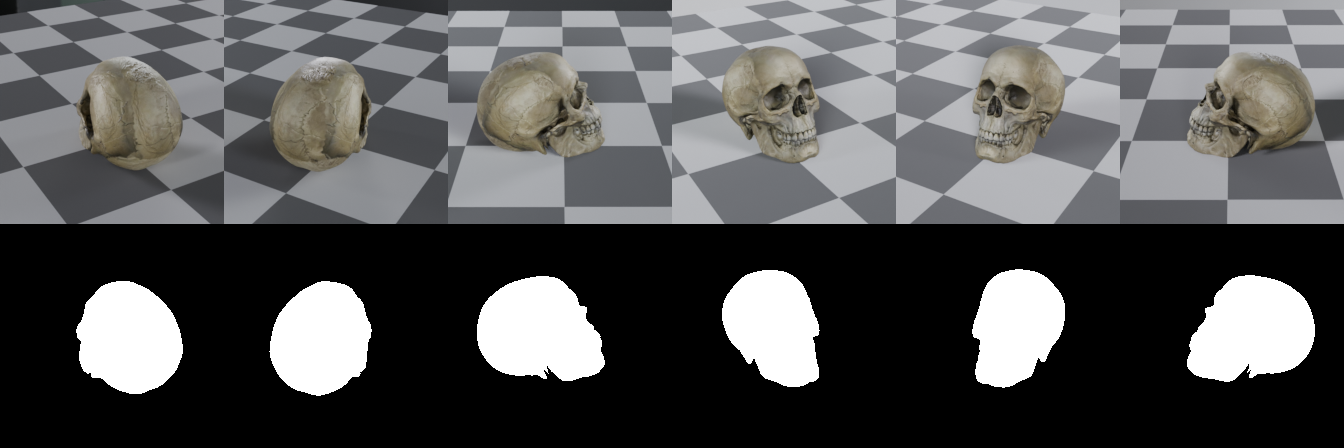
\includegraphics[width=0.8\textwidth]{skull-male-preview.png}
    \caption{Сцена 1}
    \label{fig:scene1}
\end{figure}

Рассмотрено четыре варианта настроек \texttt{COLMAP}, отличающихся уровнем
качества, использованием бинарных масок и наличием априорной калибровки камер.

\subsection{Эксперимент 0: \texttt{automatic\_reconstruction}}

Без масок и при стандартных настройках SfM уверенно восстанавливает все 200
позиций камер (рис.~\ref{fig:0sparse}), но MVS улавливает не только череп, но и
шахматный пол, образуя характерный «ковёр» из точек (рис.~\ref{fig:0fusion}).
Пустоты на верхней части модели и распыление фона наводят на мысль, что
алгоритму мешает низко‑текстурированная плоскость. Попробуем использовать маски,
чтобы ``спрятать'' фон.

% Картинки с Fusion были открыты в blender и отрендерерны как вьюпорт
% с предварительной обработкой: цвет вьюпорта изменен на белый, объекты выровнены по осям
% и в геометрии была добавлена нода "Mesh to Points", чтобы точки выглядели жирнее
\begin{figure}[h]
    \centering
    \begin{subfigure}[b]{0.3\textwidth}
        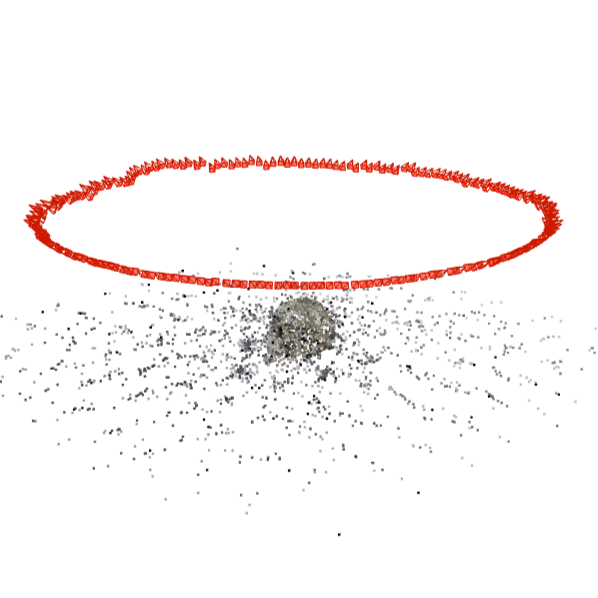
\includegraphics[width=\textwidth]{0-sparse.png}
        \caption{Sparse}
        \label{fig:0sparse}
    \end{subfigure}
    \hfill
    \begin{subfigure}[b]{0.3\textwidth}
        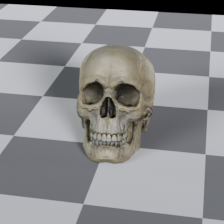
\includegraphics[width=\textwidth]{0-undistorted.png}
        \caption{Undistorted}
        \label{fig:0undistorted}
    \end{subfigure}
    \hfill
    \begin{subfigure}[b]{0.3\textwidth}
        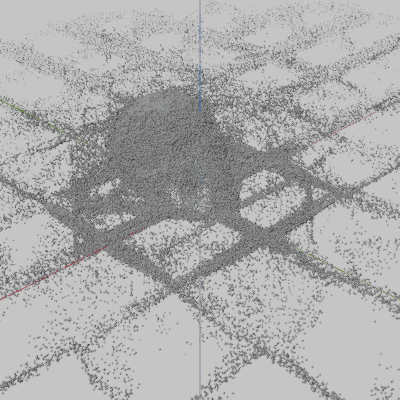
\includegraphics[width=\textwidth]{0-fusion.png}
        \caption{Fusion}
        \label{fig:0fusion}
    \end{subfigure}
    \caption{Эксперимент 0}
    \label{fig:0exp}
\end{figure}

\subsection{Эксперимент 1: \texttt{automatic\_reconstruction} + маски}

Маскирование действительно устраняет шум пола:
облако точек стало компактнее и чище
(рис.~\ref{fig:1fusion}). Однако вместе с фоном
исчезла большая чсть ключевых точек, и SfM реконструирует
лишь часть кольца камер (рис.~\ref{fig:1sparse}),
а некоторые мелкие детали черепа сглажены. Попробуем изменить настройки:
увеличить глубину поиска и число итераций, чтобы компенсировать потерю особенностей.

\begin{figure}[h]
    \centering
    \begin{subfigure}[b]{0.3\textwidth}
        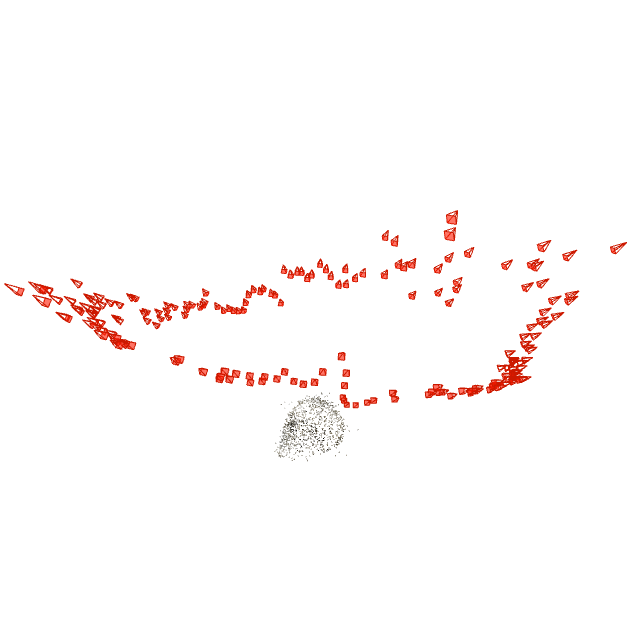
\includegraphics[width=\textwidth]{1-sparse.png}
        \caption{Sparse}
        \label{fig:1sparse}
    \end{subfigure}
    \hfill
    \begin{subfigure}[b]{0.3\textwidth}
        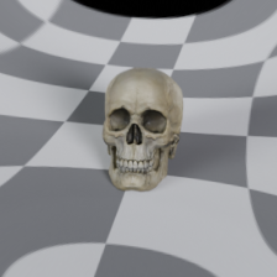
\includegraphics[width=\textwidth]{1-undistorted.png}
        \caption{Undistorted}
        \label{fig:1undistorted}
    \end{subfigure}
    \hfill
    \begin{subfigure}[b]{0.3\textwidth}
        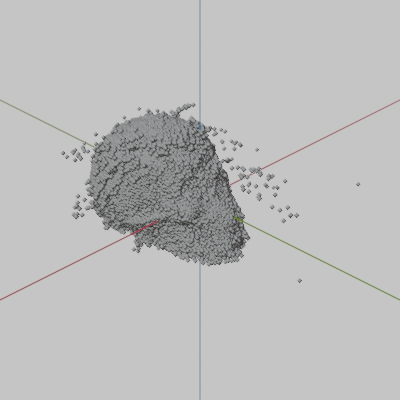
\includegraphics[width=\textwidth]{1-fusion.png}
        \caption{Fusion}
        \label{fig:1fusion}
    \end{subfigure}
    \caption{Эксперимент 1}
    \label{fig:1exp}
\end{figure}

\subsection{Эксперимент 2: \texttt{extreme} \texttt{automatic\_reconstruction} + маски}

Более агрессивные параметры возвращают почти все камеры
(рис.~\ref{fig:2sparse}), но оптимизатор ошибочно
объясняет различия в масках сильной радиальной дисторсией,
что хорошо видно по деформированному узору пола
(рис.~\ref{fig:2undistorted}). В результате
плотная модель окружена выбросами (рис.~\ref{fig:2fusion}).
Попробуем зафиксировать калибровку и позы камер
до запуска COLMAP, чтобы снять двусмысленность.

\begin{figure}[h]
    \centering
    \begin{subfigure}[b]{0.3\textwidth}
        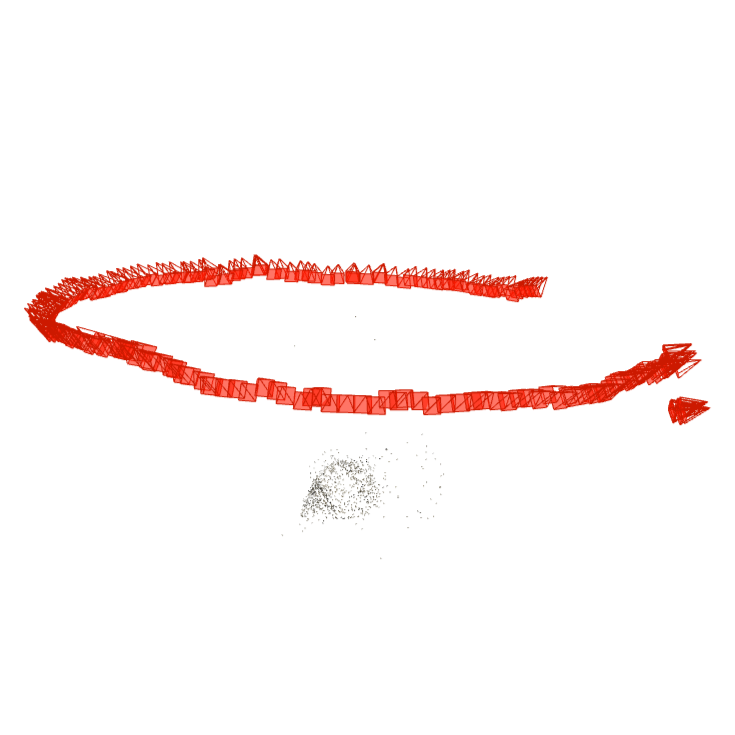
\includegraphics[width=\textwidth]{2-sparse.png}
        \caption{Sparse}
        \label{fig:2sparse}
    \end{subfigure}
    \hfill
    \begin{subfigure}[b]{0.3\textwidth}
        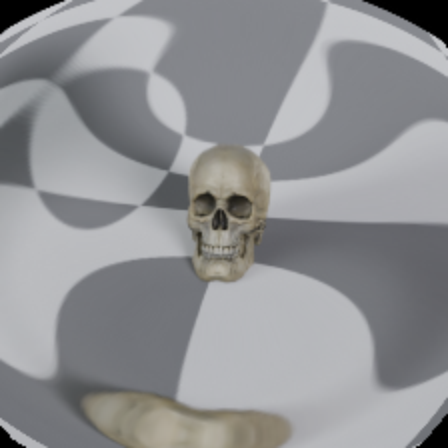
\includegraphics[width=\textwidth]{2-undistorted.png}
        \caption{Undistorted}
        \label{fig:2undistorted}
    \end{subfigure}
    \hfill
    \begin{subfigure}[b]{0.3\textwidth}
        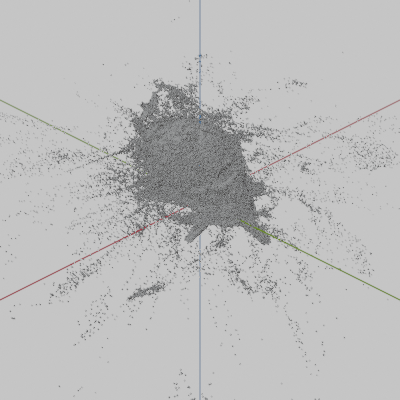
\includegraphics[width=\textwidth]{2-fusion.png}
        \caption{Fusion}
        \label{fig:2fusion}
    \end{subfigure}
    \caption{Эксперимент 2}
    \label{fig:2exp}
\end{figure}

\subsection{Эксперимент 3: априорные позы + маски, качество \texttt{extreme}}

С помощью скрипта \texttt{generate\_batch} и плагинов
\texttt{camera\_extrinsics} и \texttt{camera\_intrinsics} были получены внешние
и внутренние параметры камеры Blender. Предложенный в рамках этой работы скрипт
\texttt{to\_colmap}\footnote{Исходный код и примеры использования можно найти по
постоянной ссылке
\url{https://github.com/SherAndrei/blender-gen-dataset/tree/0a8cd30e94b21ec3442b2c315cf05be47b3b214c/scripts/to_colmap}}
позволяет заранее задать внешние и внутренние параметры камер в \texttt{COLMAP}
проекте (\texttt{cameras.txt}, \texttt{images.txt}, \texttt{database.db}), тем
самым позволяя полностью пропустить шаг с SfM.

MVS смог обеспечить наиболее плотную реконструкцию среди всех опытов
(рис.~\ref{fig:3fusion}): лобная и носовая части черепа воспроизводятся с
минимумом пропусков. Тем не менее боковые поверхности и задняя часть черепа
страдают от зеркальных бликов — в этих областях MVS по‑прежнему создаёт выбросы
и пропуски.

\begin{figure}[h]
    \centering
    \begin{subfigure}[b]{0.3\textwidth}
        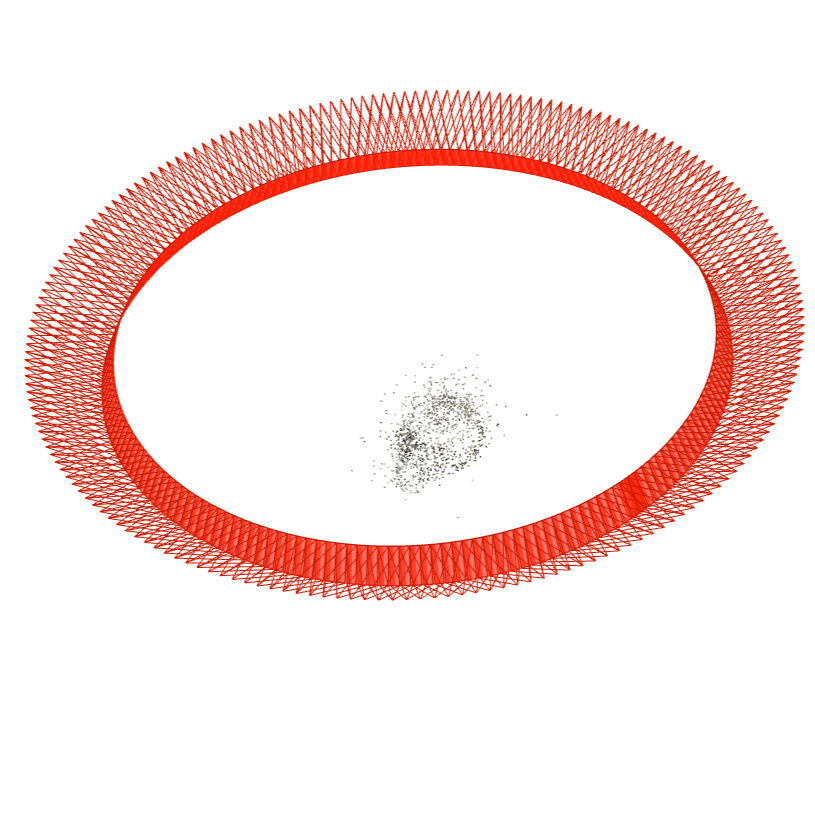
\includegraphics[width=\textwidth]{3-sparse.png}
        \caption{Sparse}
        \label{fig:3sparse}
    \end{subfigure}
    \hfill
    \begin{subfigure}[b]{0.3\textwidth}
        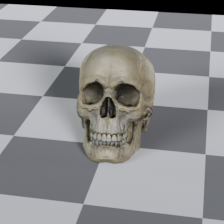
\includegraphics[width=\textwidth]{3-undistorted.png}
        \caption{Undistorted}
        \label{fig:3undistorted}
    \end{subfigure}
    \hfill
    \begin{subfigure}[b]{0.3\textwidth}
        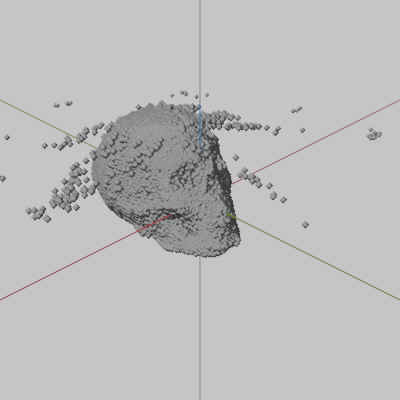
\includegraphics[width=\textwidth]{3-fusion.png}
        \caption{Fusion}
        \label{fig:3fusion}
    \end{subfigure}
    \caption{Эксперимент 3}
    \label{fig:3exp}
\end{figure}

\subsection{Эксперимент 4: Использование реальных данных}

Для проверки устойчивости классического конвейера на практическом материале был
взят видеоролик длиной 26 секунд, снятый на смартфон Samsung Galaxy A52.
Камера оставалась неподвижной, а небольшая фигурка слона из папье‑маше вращалась
на круглом пьедестале, благодаря чему получилась имитация кругового облёта
объекта. Из видеопоследовательности были извлечены сто восемьдесят восемь кадров
с частотой семь кадров в секунду с помощью программы \texttt{ffmpeg}; параметры
сжатия и оригинальное разрешение сохранены без изменений, см. рис. \ref{fig:elephant-preview}.

\begin{figure}[h]
  \centering
  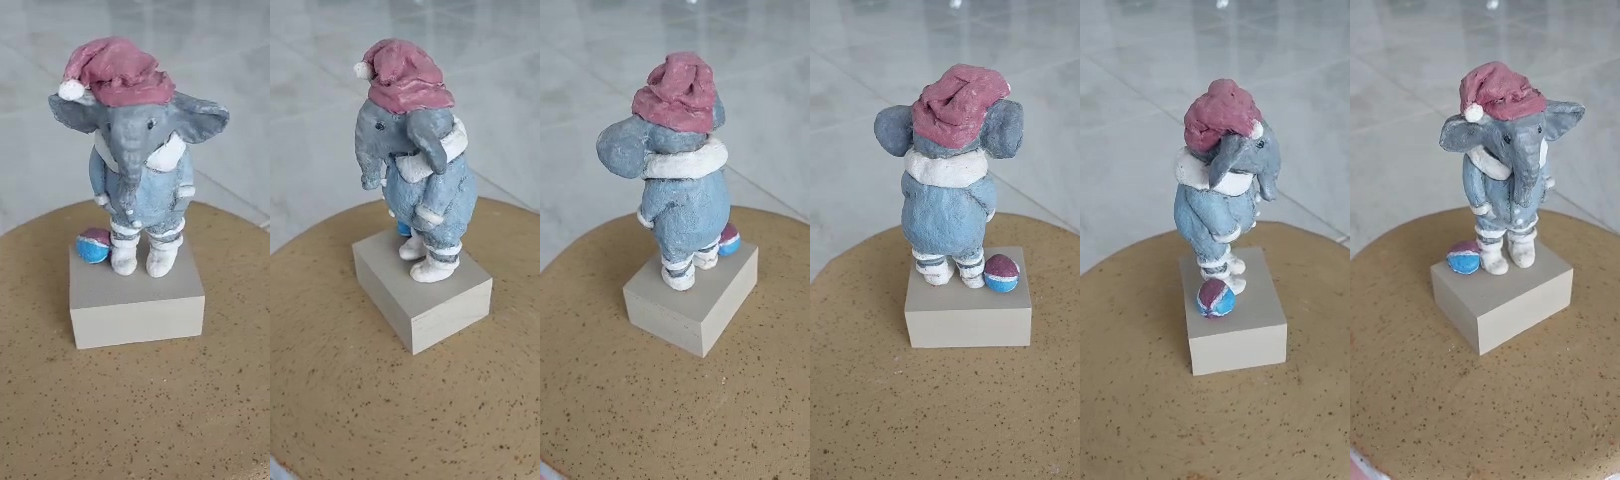
\includegraphics[width=\textwidth]{elephant-preview.png}
  \caption{Датасет фигуры из папье-маше}
	\label{fig:elephant-preview}
\end{figure}

Обработка выполнялась в \texttt{COLMAP} с использованием
\texttt{automatic\_reconstruction} с уровнем качества \texttt{extreme}. В
качестве оптимизации задействован \texttt{sequential\_matcher}, а также
указано использование единственной камеры. Полный
цикл «SfM + MVS» занял чуть больше 32 двух минут на рабочей станции.

\begin{figure}[h]
    \centering
    \begin{subfigure}[b]{0.3\textwidth}
        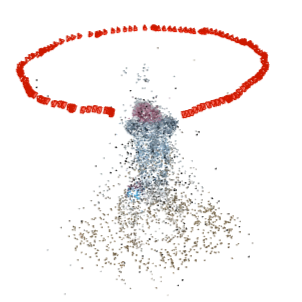
\includegraphics[width=\textwidth]{4-sparse.png}
        \caption{Sparse}
        \label{fig:4sparse}
    \end{subfigure}
    \begin{subfigure}[b]{0.3\textwidth}
        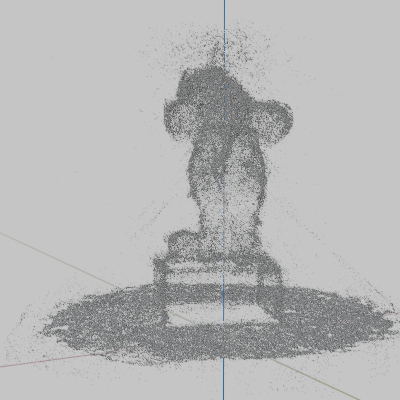
\includegraphics[width=\textwidth]{4-fusion.png}
        \caption{Fusion}
        \label{fig:4fusion}
    \end{subfigure}
    \caption{Эксперимент 4}
    \label{fig:4exp}
\end{figure}

Полученная разреженная модель показала, что алгоритм и корректно восстановил
замкнутую траекторию камер, и определил положение фигурки без заметных
отклонений. Обилие текстурных элементов на отдалённом фоне дополнительно
стабилизировало процесс bundle adjustment и снизило вероятность вырождения
оптимизации. Плотное облако точек, полученное после этапа fusion, содержало
выраженную «корону» из шумовых точек по периметру модели. Этот артефакт был
вызван теми же фон‑специфичными признаками, которые помогали SfM, — при переходе
к MVS они оказались ошибочно привязанными к объекту интереса, см. \ref{fig:floor-as-feature}.

\begin{figure}[h]
    \centering
    \begin{subfigure}[b]{0.2\textwidth}
        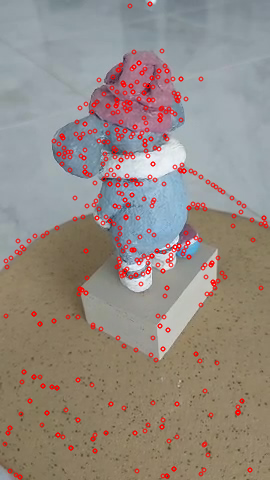
\includegraphics[width=\textwidth]{0-floor-as-feature.png}
    \end{subfigure}
    \begin{subfigure}[b]{0.2\textwidth}
        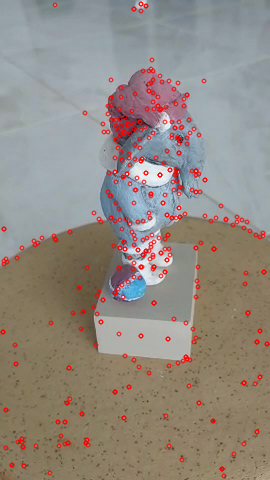
\includegraphics[width=\textwidth]{1-floor-as-feature.png}
    \end{subfigure}
    \caption{Пол считается частью объекта}
    \label{fig:floor-as-feature}
\end{figure}

Качество реконструкции оказалось сопоставимо с самым первым синтетическим
опытом: геометрия слона читается, однако детализация заметно ухудшена за счёт
шумов. Основной вывод заключается в том, что даже при съёмке на обычный смартфон
и при отсутствии строгого контроля за сценой классический алгоритм способен
обеспечить полноценную трёхмерную реконструкцию. При этом главной проблемой
остаётся борьба с фоновой информацией: либо сцену следует подготавливать, либо
необходимо применять очистку плотного облака.

\subsection{Выводы}

Разбор последовательных экспериментов позволяет выделить
устойчивые особенности работы классической связки SfM+MVS:

\begin{itemize}
    \item При богатой текстуре и отсутствии масок метод уверенно восстанавливает
    кольцевую траекторию камер и создаёт приемлемую плотность модели.

    \item Маскирование удаляет шум пола и делает облако чище, но одновременно
    обедняет граф соответствий; часть камер не восстанавливается, а мелкие
    детали сглаживаются.

    \item Изменение настроек алгоритмов компенсирует нехватку патчей,
    однако без жёсткой калибровки маски интерпретируются как радикальная
    дисторсия, что приводит к расплыванию геометрии.

    \item Предварительно зафиксированные интринзики и позы снимают
    неоднозначность и дают лучший баланс плотности и чистоты, однако зеркальные
    блики и самоокклюзии всё ещё рождают выбросы и пробелы — предел классической
    фотограмметрии.
\end{itemize}

\noindent Чтобы преодолеть ограничения классической фотограмметрии — зеркальные
блики, маски, скудную текстуру и самоокклюзии — необходима более выразительная
регуляризация. Именно её предлагают современные нейронные методы (NeRF, TensoRF
и др.). В следующей главе мы последовательно разберём эти архитектуры, покажем,
каким образом они используют параметры камер, полученные SfM, и сравним их
результаты с классическим подходом на тех же тестовых сценах.

\section{Тензорные поля излучения}

В 2020 году модель \emph{Neural Radiance Fields} (NeRF) впервые показала, что по
набору фотографий и поз камер можно восстановить непрерывную функцию, которая
для любой точки пространства возвращает плотность $\sigma$ и цвет $\mathbf{c}$.
Решение хранилось внутри большого MLP, обучавшегося днями на одну сцену и
требовавшего сотни мегабайт памяти.

Необходимость ускорить обучение и снизить потребление памяти
привела к идее компактных представлений.
Ответом стал \emph{TensoRF} (2022):
он сохраняет саму формулировку задачи NeRF: «какой цвет и какая плотность
в каждой точке?», но заменяет тяжёлый MLP на низкоранговую
\emph{тензорную факторизацию} радианс‑поля.

Вместо полного 3D массива $D_x\times D_y\times D_z$ TensoRF хранит три набора
«полосок» вдоль осей $X$, $Y$, $Z$.  Память падает с $\mathcal{O}(D^3)$ до
$\mathcal{O}(3RD)$, где $R$ — ранг разложения. Из‑за малого числа параметров
(обычно $\sim10^6$ против $\sim10^8$ у NeRF) обучение одной сцены занимает
десятки минут на GPU.

TensoRF ``подхватил'' идею NeRF описывать сцену непрерывной функцией, но
переформулировал хранение этой функции как низкоранговую таблицу умножения
одномерных векторов.  В результате добился сопоставимого качества при
существенно меньших вычислительных и временных затратах.

Для оценки реальных возможностей TensoRF мы провели
четыре последовательных эксперимента\footnote{Код
и конфигурационные файлы доступны в репозитории проекта по ссылке \url{https://github.com/SherAndrei/3d-reconstruction}.}.
Результат работы модели оценивается с помощью метрики PSNR (англ. \emph{Peak signal-to-noise ratio}),
чем выше результат которой, тем лучше, приемлемыми считаются значения больше 30 дБ.

\subsection{Эксперимент 0: Диффузный объект}
Сцена — уже известная 3D модель черепа; датасет из 200 фотографий, сгенерированных скриптом
\texttt{generate\_batch} с масками, заранее задами позами и внутренними
параметрами камер. Разбиение: 150 кадров в train, 50 в test.  Обучение на GPU
Tesla T4 заняло $10$ минут; получена средняя $\operatorname{PSNR} = 44.26$ дБ.

\begin{figure}[h]
  \centering
  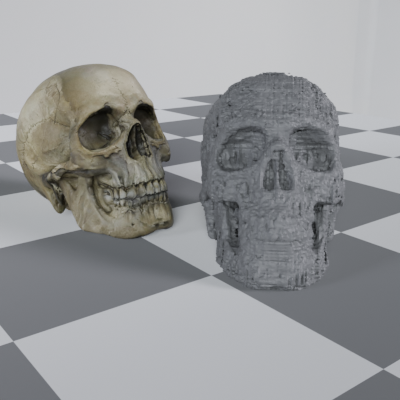
\includegraphics[width=0.3\textwidth]{tensorf-skull.png}
  \caption{Восстановленная модель черепа рядом с оригинальной}
\end{figure}

\subsection{Эксперимент 1: Драгоценный камень в макросъёмке}
Аналогичный набор с заранее известными позами камер из 200 кадров размера
$400\times400$~px представлен на рис.  \ref{fig:asscher-preview}, Сцену
составляет прозрачный огранённый камень в сравнимых с реальным драгоценным
камнем в размерах, из-за чего съёмка виртуальной камерой производится с большим
фокусным расстоянием (камень занимает почти весь кадр).

\begin{figure}[h]
  \centering
  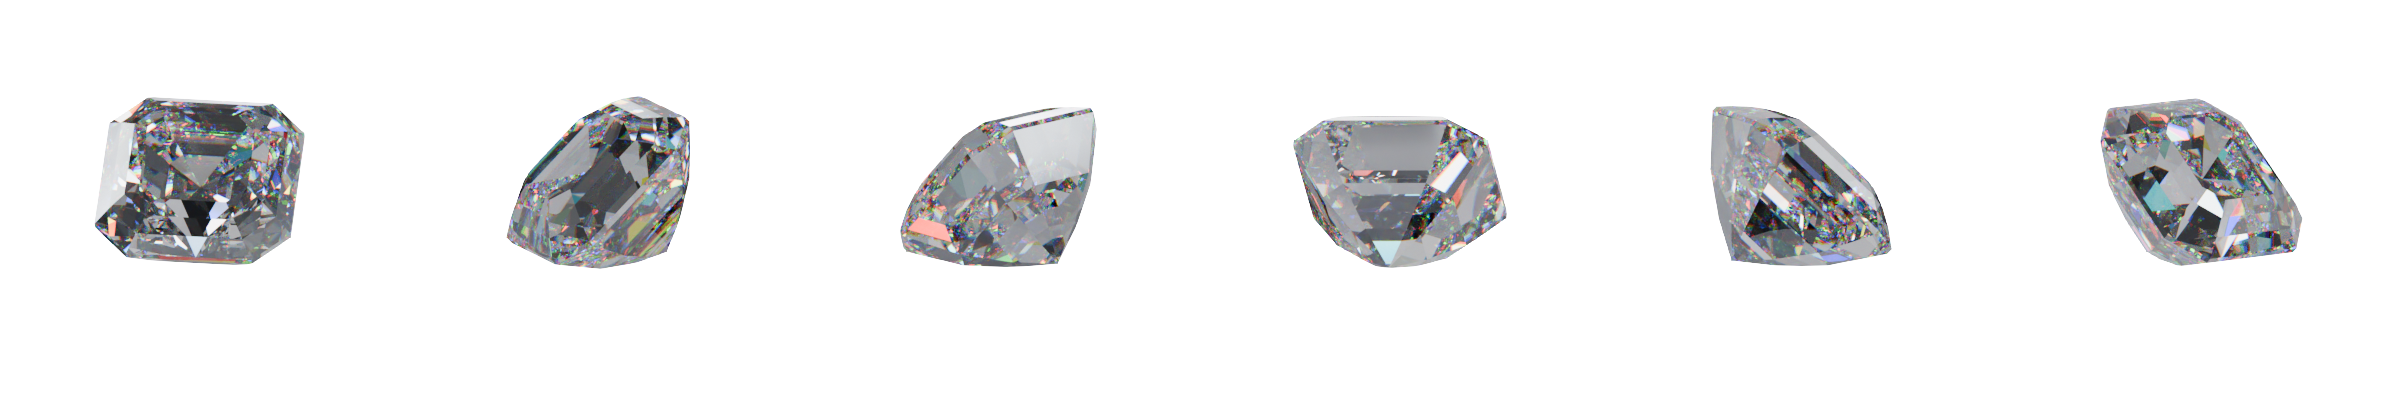
\includegraphics[width=0.8\textwidth]{diamond-asscher-masked-preview.png}
  \caption{Используемый датасет драгоценного камня}
	\label{fig:asscher-preview}
\end{figure}

TensoRF выдал заметно худший результат $\operatorname{PSNR}=23.13$ дБ; на
рис.~\ref{fig:tensorf-asscher-small} видно искажение — модель не распознала
реальный микроскопический масштаб и сформировала лишь размытый объём с шумом.

\subsection{Эксперимент 2: «Обман масштаба».}
Чтобы проверить гипотезу о влиянии масштаба сцены, с помощью
\texttt{generate\_batch} были сгенерированы соответствующие позы и внутренние
параметры камер, совпадающие с параметрами, которые использовались для
черепа\footnote{Обращаю внимание, что так как размер изображения драгоценного
камня отличается от размера изображения черепа, то отличаются и внутренние
параметры у камер, поэтому генерацию нужно проделывать заново.}.
Новые параметры подложили в датасет с изображениями бриллианта.
При тех же настройках обучения удалось получить приемлемое качество, $\operatorname{PSNR}=29.17$
(cм. рис.~\ref{fig:tensorf-asscher-large}).


\begin{figure}[h]
    \centering
    \begin{subfigure}[h]{0.45\textwidth}
      \centering
      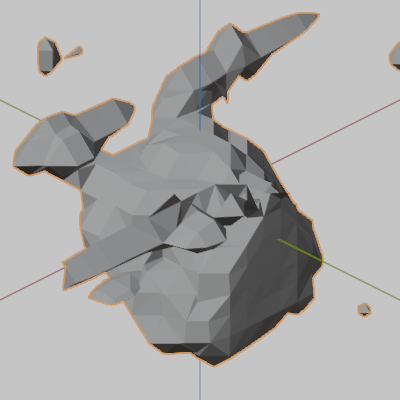
\includegraphics[width=0.6\textwidth]{tensorf-asscher-small.png}
      \caption{Неудачная попытка восстановления}
      \label{fig:tensorf-asscher-small}
    \end{subfigure}\hfill
    \begin{subfigure}[h]{0.45\textwidth}
     \centering
      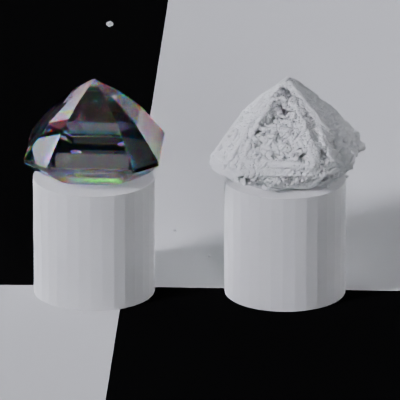
\includegraphics[width=0.6\textwidth]{tensorf-asscher-large.png}
      \caption{Восстановленный драгоценный камень}
      \label{fig:tensorf-asscher-large}
    \end{subfigure}
    \caption{}
\end{figure}

Тем не менее прозрачная структура
привела к локальным пустотам внутри тела,
что косвенно указывает на сложности модели
с реконструкцией стекло‑подобных материалов.

\subsection{Эксперимент 3: Использование реальных данных}

В качестве входных данных использовался тот же видеоролик с фигуркой
слонёнка, что и в соответствующем классическом эксперименте.
Датасет был разбит на две части: 141 кадр в трейн‑выборке
и 46 кадров в тестовой. Поскольку COLMAP ранее уже оценил
внешние и внутренние параметры камеры, эти калибровочные
данные были напрямую переиспользованы в процессе обучения TensoRF.

Главное отличие от синтетических примеров заключается в отсутствии
бинарных масок: TensoRF должен самостоятельно «догадаться»,
где заканчивается объект и начинается фон. По умолчанию
алгоритм ограничивает область поиска коробкой
$\verb|scene_bbox|$ с координатами от $(-1.5,-1.5,-1.5)$
до $(1.5,1.5,1.5)$. Однако фигурка вместе с пьедесталом в эти
границы не помещалась: часть модели обрезалась, что хорошо видно
на левом фрагменте рис.~\ref{fig:tensorf_real}.

\begin{figure}[h]
    \centering
    \begin{subfigure}[b]{0.45\textwidth}
        \centering
        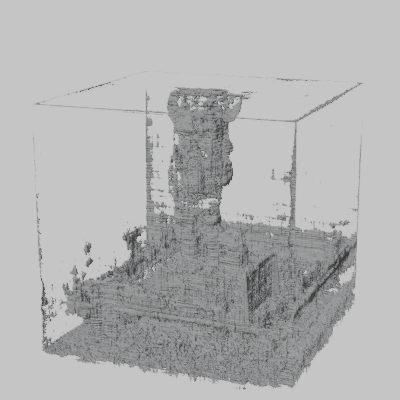
\includegraphics[width=0.6\textwidth]{tensorf-elephant-bad-bbox.png}
        \caption{До настройки параметров}
    \end{subfigure}\hfill
    \begin{subfigure}[b]{0.45\textwidth}
        \centering
        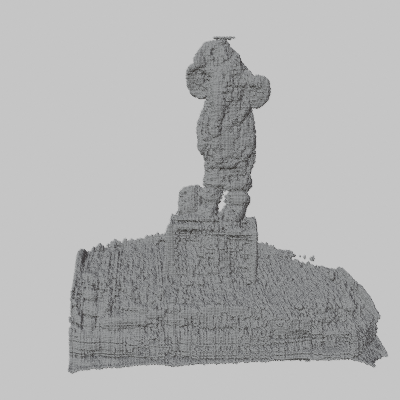
\includegraphics[width=0.6\textwidth]{tensorf-elephant.png}
        \caption{После настройки}
    \end{subfigure}
    \caption{Влияние настройки \texttt{scene\_bbox} и \texttt{near\_far}.}
    \label{fig:tensorf_real}
\end{figure}

Чтобы учесть истинные габариты сцены, границы коробки были
расширены до $[-2,2]^3$. Дополнительно изменён диапазон
$\verb|near_far|$ c $[0.1,100]$ до $[1.0,6.0]$.
Параметр \texttt{near\_far} задаёт ближнюю и дальнюю плоскости
отсечения, внутри которых происходит интегрирование вдоль лучей.
Сужая диапазон, мы исключили участок пола, расположенный
за объектом.

После внесения правок и запуска оптимизации на 5000 итераций\footnote{В
контексте TensoRF «итерация» — это один шаг стохастического градиентного спуска,
в котором мини‑батч лучей используется для обновления параметров тензорных
решёток.} за 40 минут метрика PSNR на валидационных изображениях достигла $34.7$ дБ, а
результирующая трёхмерная модель (правый фрагмент рис.~\ref{fig:tensorf_real})
приобрела чёткий силуэт без шумов и обрезанных частей. Таким образом, даже без
масок TensoRF способен реконструировать объект из реального видео, если
предварительно корректно задать габариты сцены и границы интегрирования по лучу.

\chapter{Заключение}

В данной работе была поставлена цель разработать методику восстановления
трёхмерных моделей объектов в сложных сценах. Для её
достижения были сформулированы три задачи: аналитический обзор методов
3D-реконструкции, поиск и подготовка подходящих наборов данных, а также
экспериментальное сравнение традиционных и нейросетевых алгоритмов на этих
данных. В рамках исследования все перечисленные задачи выполнены.

Во‑первых, проведён подробный обзор отечественных и зарубежных публикаций,
охватывающий эволюцию методов от стереозрения и MVS до генеративных нейросетевых
моделей и неявных представлений поверхностей. Анализ позволил систематизировать
преимущества и ограничения подходов и выделить критерии, критически важные для
сложных сцен: требуемый объём входных данных, точность геометрии, устойчивость
к шуму и время вычислений.

Во‑вторых, решена проблема дефицита открытых датасетов для сцен с богатой
геометрией и неконтролируемыми условиями съёмки. Для этого разработан
конфигурируемый скрипт \texttt{generate-batch.py}, использующий Blender, с
системой плагинов, автоматически генерирующий изображения, глубину, нормали,
маски и полные параметры камеры. Дополнительный скрипт \texttt{to\_colmap}
переводит синтетические в формат COLMAP, что обеспечивает совместимость с
классическими алгоритмами SfM. Открытость и документированность инструментов
позволяют быстро формировать собственные выборки и повторять эксперименты.

В‑третьих, проведена серия воспроизводимых экспериментов. Классический конвейер
SfM+MVS и современная модель TensoRF протестированы на двух типах данных: (i)
синтетических сценах с огранённым драгоценным камнем и археологическим
объектом; (ii) наборе фотографий, снятых смартфоном. Полученные результаты
показывают, что:

\begin{itemize}
  \item при достаточном числе ракурсов и точной калибровке камеры TensoRF даёт заметно
  более высокие показатели PSNR по сравнению с MVS, позволяя восстановить
  мелкие детали и сократить ручную пост‑обработку;
  \item в условиях ограниченного набора снимков и отсутствия масок классическая
  фотограмметрия остаётся конкурентоспособной по времени и стойкости
  к артефактам;
  \item использование синтетических фотосессий, сгенерированных описанным скриптом,
  упрощает тонкую настройку нейросетевой модели и позволяет уменьшить объём
  реальных данных, необходимых для обучения.
\end{itemize}

Таким образом, предложена практическая методика, подтверждённая экспериментами,
и создан набор инструментов для её дальнейшего применения и развития.

Инструментарий и рекомендации, разработанные в работе, могут быть использованы
для оценки качества огранки драгоценных камней, цифровой архивации
археологических находок, а также в смежных областях, где требуется точное или
быстродействующее восстановление геометрии при ограниченном доступе
к сканирующему оборудованию.

Полученная методика пока не рассматривает прозрачные и сильно отражающие
поверхности, а также не оптимизирована под реконструкцию в реальном времени.

Реализация этих направлений позволит ещё более широко применять предложенную
методику в практике инженерных, культурно‑исторических и медицинских задач.

\include{10-attachments}

\printbibliography

\end{document}
